% AI-translated component: printed 292--301.
% Principal PDF 299--308; Google 303--308, 309--310; HKUST pg00306--307 for 298--299.
\begingroup
\newcommand{\IXarc}[1]{\overset{\frown}{#1}}
\clearpage
\noindent 292\hfill\textsc{Remarks.}\hfill\mbox{}\par\medskip
\noindent If, on the other hand, $A.1$ had been measured, the azimuth would be $1-A.1$. If point $A$ is also linked to another principal direction, for example to 2, we have
\[
\begin{aligned}
A'&=1+1.A\\
A''&=2+2.A.
\end{aligned}
\]
If both determinations give the same value for $A$, no further calculation is of course necessary. Otherwise one takes the mean of the two, allowing for their different weights. For if $1.A$ had been measured $p'$ times by repetition and $2.A$ had been measured $p''$ times, the most probable value would be $A=\dfrac{A'p'+A''p''}{p'+p''}$.

Each day's measurements must without exception be entered in ink on the same day. \textsc{Gauss}, however, records the mean of all the vernier readings directly instead of giving the individual readings. His log takes the following form:
\begin{center}
(1833) 21 Sept. \textls[100]{Wittekindstein.}\\
The air clear and pure.\\
Hünenburg --- Nonnenstein

\smallskip
{\footnotesize
\setlength{\tabcolsep}{3pt}
\begin{tabular}{c|c|c|c}
\multicolumn{1}{c}{(Rep.)}&
\multicolumn{1}{c}{(reading)}&
\multicolumn{1}{c}{(5-fold angle)}&
\multicolumn{1}{c}{(single angle obtained from all readings)}\\
0 &$113^\circ\ 5'\ 19''{,}250$&&\\
5 &$341\ 18\ 40{,}725$&$228^\circ13'\,21''{,}475$&\\
10&$209\ 32\ \phantom{0}0{,}050$&$19{,}325$&\\
15&$\phantom{0}77\ 45\ 18{,}125$&$18{,}075$&\\
20&$305\ 58\ 43{,}750$&$25{,}625$&$45^\circ38'\,40''{,}225$\\
\multicolumn{4}{c}{etc.}
\end{tabular}}
\end{center}
\textsc{Gauss} also adjusted the angles and drew up the first table at the stations themselves. This table is prepared as follows. Once a provisional orientation has been set and the principal directions have been adjusted, the azimuths of all the objects sighted for intersection are calculated by the method given above and arranged in order of magnitude. The table thus takes the following form:
\begin{center}
\textls[120]{Wittekindstein}\\[3pt]
\begin{tabular}{l@{\quad}r@{\;}r@{\;}r}
\multicolumn{4}{c}{\makebox[8.4cm]{.\hfill.\hfill.\hfill.\hfill.\hfill.\hfill.\hfill.\hfill.\hfill.\hfill.\hfill.\hfill.\hfill.\hfill.\hfill.\hfill.\hfill.\hfill.\hfill.\hfill.\hfill.\hfill.\hfill.\hfill.\hfill.\hfill.\hfill.\hfill.\hfill.\hfill.\hfill.\hfill.\hfill.\hfill.\hfill.\hfill.\hfill.}}\\
\textit{Deister}&270&29&$32{,}770$\\
Hattendorf&273&3&$53{,}768$\\
\textit{Pagenburg}&282&57&$28{,}391$\\
Schaumburg (small red pinnacle)&283&43&$54{,}766$\\
Schaumburg (higher pinnacle)&283&55&$39{,}766$\\
\multicolumn{1}{c}{etc.}&\multicolumn{3}{c}{etc.}
\end{tabular}
\end{center}
\noindent\hbox to0pt{\raisebox{.3ex}{\scriptsize--}\hss}%
\par
The points written in italics indicate the principal directions.

For principal triangulation points and secondary points alike, it will often happen that the point sighted from other stations cannot serve as the instrument station, because the site does not allow the instrument to be set up there. In such a case a suitable point nearby must be chosen for setting up the instrument, and a centering correction must then be made so that the directions taken from the other stations to the point in question can be compared with the angles measured here. This centering correction can be applied in two ways, either by correcting the azimuths \textls[150]{toward the point} so

\clearpage
\noindent\mbox{}\hfill\textsc{Station Adjustments.}\hfill293\par\medskip
\noindent that they refer to the instrument station, or by reducing the angles measured from the instrument station to the target point. It is simplest, however, to center the azimuths derived from the measured angles rather than the angles themselves. To carry out the centering one must know the so-called centering elements, that is, the distance from the instrument station to the target point and the azimuth of this direction. If 1 is the target point, 2 the instrument station, and $P$ the more distant point that was sighted, then, denoting azimuths by a $\frown$ above them and distances by ---, we have:
\[
\begin{aligned}
\IXarc{2P}&=\IXarc{1P}+\frac{206265''\cdot\overline{21}}{\overline{2P}}\sin(\IXarc{1P}-\IXarc{12})
=\IXarc{1P}+\frac{206265''\cdot\overline{21}}{\overline{2P}}\sin(\IXarc{21}-\IXarc{1P})\\[4pt]
&=\IXarc{1P}+\frac{206265''\cdot\overline{21}}{\overline{1P}}\sin(\IXarc{2P}-\IXarc{12})
=\IXarc{1P}+\frac{206265''\cdot\overline{21}}{\overline{1P}}\sin(\IXarc{21}-\IXarc{2P}),
\end{aligned}
\]
where, of course, the lengths $\overline{21}$, $\overline{1P}$ or $\overline{21}$, $\overline{2P}$ must be measured in the same units. This reduction therefore requires knowledge of the length $\overline{1P}$ or $\overline{2P}$. Since this length is determined definitively only from measurements at both stations, one seems to be reasoning in a circle here. But the correction $\dfrac{206265''\cdot\overline{21}}{\overline{2P}}\sin(\IXarc{1P}-\IXarc{12})$ will always be very small, since the ratio $\dfrac{\overline{21}}{\overline{2P}}$ is very small. An approximate value of $\overline{1P}$, which can always be obtained without knowing the measurements at 2, is therefore sufficient to determine the correction. ---

Calculating the centering correction thus presents no difficulty once the centering elements are known. Determining these elements may in some cases involve difficulties, and nothing can be said about it in general. The observer must find the most suitable method in each case. We consider here only the case where one can actually measure from 1 to 2. \textsc{Gauss} then determines the azimuth by placing a fine object, such as a pin, over the center of the theodolite. He then brings his eye into line with the pin and point 2 and notes the point on the horizon that corresponds to this direction. If there is no suitable object there, he has his assistant set up a pole. He then measures the angle between any principal point visible from 1 and this pole, thereby obtaining the azimuth of 2. Knowing it to within 2--4 arcminutes is sufficient in almost all cases. If this procedure cannot be used, perhaps because 2 is not visible from 1, one chooses two points $s$, $s'$ from which 1 and 2 can be seen and sights 1 and 2 from those points. The orientation at the two chosen points can be found by sighting them for intersection from 1. By then measuring the distance $ss'$, one obtains by a simple calculation the positions of 1 and 2 relative to $s$, $s'$, and from these both $\overline{12}$ and $\IXarc{12}$.«

\medskip
A few slips of the pen have been corrected in the letters to \textsc{Schumacher} under [6].

\hfill\textsc{Krüger.}
\vfill
\begin{center}\rule{4cm}{.4pt}\end{center}

% Unnumbered blank leaf, contextual printed 294.
\clearpage\null
% Unnumbered title leaf, contextual printed 295.
\clearpage
\vspace*{\fill}
\begin{center}{\LARGE ON NETWORK ADJUSTMENT.}\end{center}
\vfill
% Unnumbered blank leaf, contextual printed 296.
\clearpage\null
% Unnumbered opening leaf, contextual printed 297.
\clearpage
\begin{center}
{\Large POSTHUMOUS PAPERS AND CORRESPONDENCE.}\\[2cm]
[1.]\\[3pt]
[Number of Condition Equations in a Triangulation System.]
\end{center}
A system of $p$ points connected by $l$ lines gives
\[
\begin{aligned}
l-p+1\quad&\text{condition equations from angular relations,}\\
l-2p+3\quad&\text{from side ratios, thus in all}\\
2l-3p+4.&
\end{aligned}
\]
\noindent\llap{.\hspace{1em}}\indent For the measurements of 1824, $p=13$, $l=29$, giving 17 and 6 condition equations respectively.

For the whole system, $p=33$, $l=75$. We therefore have
\begin{quote}
43 condition equations of the first kind,\\
12 condition equations of the second kind.
\end{quote}
\begin{center}
[2.]\\[3pt]
The 33 principal triangulation points and their connections.
\end{center}
\noindent
\begin{tabular}{r|l|l}
1&Göttingen&$1\,.\,.\,.\,2.\,3$\\
2&Merid. mark&$2\,.\,.\,.\,1.\,3.\,4$\\
3&Hohehagen&$3\,.\,.\,.\,1.\,2.\,4.\,5.\,6$\\
4&Hils&$4\,.\,.\,.\,2.\,3.\,5.\,7.\,8$\\
5&Brocken&$5\,.\,.\,.\,3.\,4.\,6.\,7$\\
6&Inselsberg&$6\,.\,.\,.\,3.\,5$\\
7&Lichtenberg&$7\,.\,.\,.\,4.\,5.\,8.\,9.\,10$\\
8&Deister&$8\,.\,.\,.\,4.\,7.\,9.\,10$\\
9&Garssen&$9\,.\,.\,.\,7.\,8.\,10.\,11$\\
10&Falkenberg&$10\,.\,.\,.\,7.\,8.\,9.\,11.\,12.\,13.\,14.\,15.\,19$
\end{tabular}
\vfill
\noindent{\small IX.}\hfill38

\clearpage
\noindent298\hfill\textsc{Posthumous Papers.}\hfill\mbox{}\par\bigskip
\noindent
\begin{tabular}{r|l|l}
11&Scharnhorst&$11\,.\,.\,.\,9.\,10.\,12$\\
12&Breithorn&$12\,.\,.\,.\,10.\,11.\,13.\,15$\\
13&Hauselberg&$13\,.\,.\,.\,10.\,12.\,14.\,15$\\
14&Wulfsode&$14\,.\,.\,.\,10.\,13.\,15.\,16$\\
15&Wilsede&$15\,{,}\,.\,.\,10.\,12.\,13.\,14.\,16.\,17.\,\tikz[baseline=0pt,x=1em,y=1em]{\fill (0,.65) rectangle (.12,.79);\draw[line width=.5pt] (0,-.12)..controls(.08,-.15)..(.15,-.12);}\!18.\,19.\,20.\,21.\,22.\,23.\,24.\,25.\,26$\\
16&Timpenberg&$16\,.\,.\,.\,14.\,15.\,17.\,21$\\
17&Nindorf&$17\,.\,.\,.\,15.\,16.\,18.\,21$\\
18&Lüneburg&$18\,.\,.\,.\,15.\,17.\,21$\\
19&Elmhorst&$19\,.\,.\,.\,10.\,15.\,20.\,22$\\
20&Litberg&$20\,.\,.\,.\,15.\,19.\,21.\,23.\,25$\\
21&Hamburg&$21\,.\,.\,.\,15.\,16.\,17.\,18.\,20$\\
22&Bullerberg&$22\,.\,.\,.\,15.\,19.\,23.\,24$\\
23&Brüttendorf&$23\,.\,.\,.\,15.\,20.\,22.\,24.\,25.\,27$\\
24&Bottel&$24\,.\,.\,.\,15.\,22.\,23.\,26.\,27$\\
25&Zeven&$25\,.\,.\,.\,15.\,20.\,23.\,26.\,27.\,28$\\
26&Steinberg&$26\,.\,.\,.\,15.\,24.\,25.\,27$\\
27&Bremen&$27\,.\,.\,.\,23.\,24.\,25.\,26.\,28.\,29$\\
28&Brillit&$28\,.\,.\,.\,25.\,27.\,29.\,30$\\
29&Garlste&$29\,.\,.\,.\,27.\,28.\,30.\,31$\\
30&Bremerlehe&$30\,.\,.\,.\,28.\,29.\,31.\,32$\\
31&Varel&$31\,.\,.\,.\,29.\,30.\,32.\,33$\\
32&Langwarden&$32\,.\,.\,.\,30.\,31.\,33$\\
33&Jever&$33\,.\,.\,.\,31.\,32.$
\end{tabular}

\clearpage
\noindent\mbox{}\hfill\textsc{On Network Adjustment.}\hfill299\par\smallskip
\begin{center}
% Coordinates follow the principal map; all edges terminate at the named shared node.
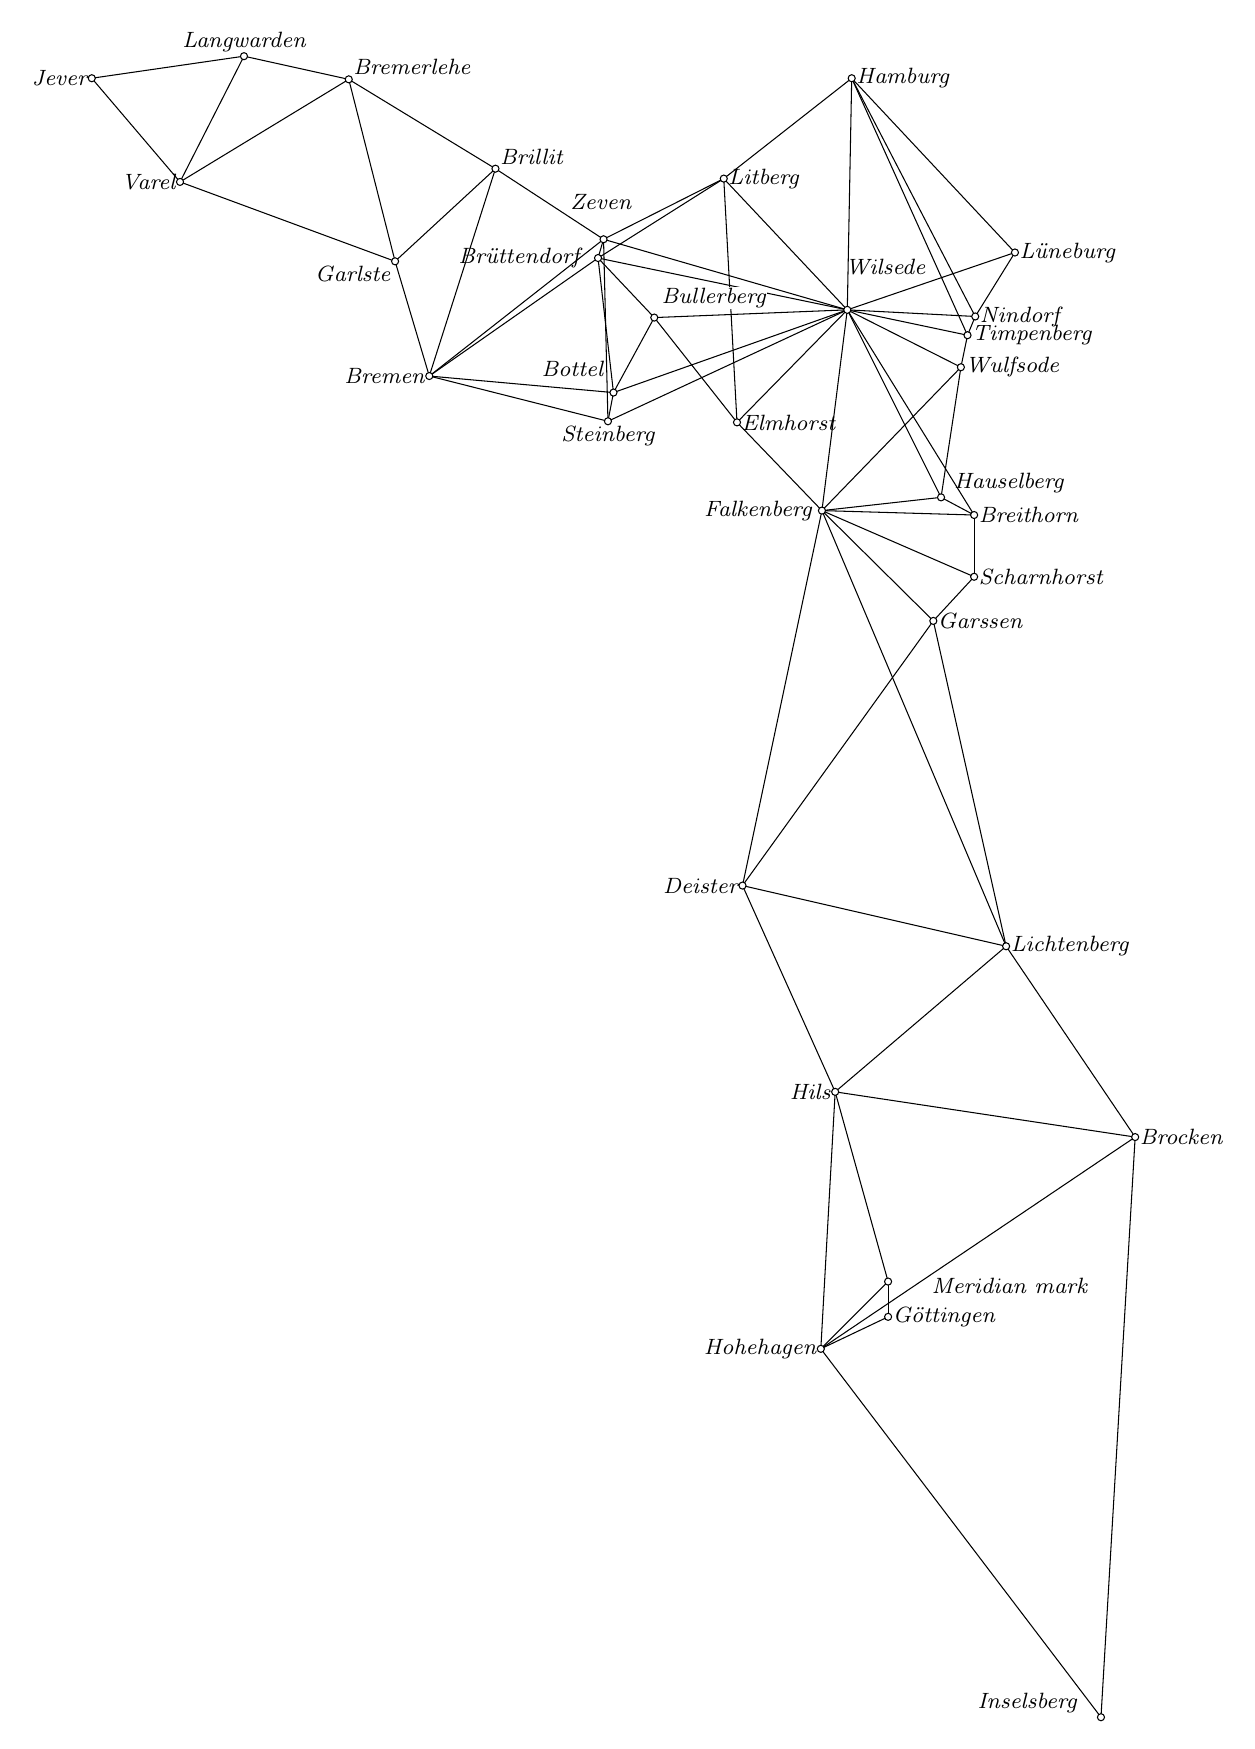
\begin{tikzpicture}[x=.014cm,y=-.014cm,line width=.38pt,
 every node/.style={font=\footnotesize\itshape,inner sep=1.5pt}]

\coordinate (n1) at (907,1341);
\coordinate (n2) at (907,1309);
\coordinate (n3) at (846,1370);
\coordinate (n4) at (859,1137);
\coordinate (n5) at (1131,1178);
\coordinate (n6) at (1100,1704);
\coordinate (n7) at (1014,1005);
\coordinate (n8) at (775,950);
\coordinate (n9) at (948,710);
\coordinate (n10) at (847,610);
\coordinate (n11) at (985,670);
\coordinate (n12) at (985,614);
\coordinate (n13) at (955,598);
\coordinate (n14) at (973,480);
\coordinate (n15) at (870,428);
\coordinate (n16) at (979,451);
\coordinate (n17) at (986,434);
\coordinate (n18) at (1022,376);
\coordinate (n19) at (770,530);
\coordinate (n20) at (758,309);
\coordinate (n21) at (874,218);
\coordinate (n22) at (695,435);
\coordinate (n23) at (644,381);
\coordinate (n24) at (658,503);
\coordinate (n25) at (649,364);
\coordinate (n26) at (653,529);
\coordinate (n27) at (491,488);
\coordinate (n28) at (551,300);
\coordinate (n29) at (460,384);
\coordinate (n30) at (418,219);
\coordinate (n31) at (265,312);
\coordinate (n32) at (323,198);
\coordinate (n33) at (185,218);
\draw (n1) -- (n2);
\draw (n1) -- (n3);
\draw (n2) -- (n3);
\draw (n2) -- (n4);
\draw (n3) -- (n4);
\draw (n3) -- (n5);
\draw (n3) -- (n6);
\draw (n4) -- (n5);
\draw (n4) -- (n7);
\draw (n4) -- (n8);
\draw (n5) -- (n6);
\draw (n5) -- (n7);
\draw (n7) -- (n8);
\draw (n7) -- (n9);
\draw (n7) -- (n10);
\draw (n8) -- (n9);
\draw (n8) -- (n10);
\draw (n9) -- (n10);
\draw (n9) -- (n11);
\draw (n10) -- (n11);
\draw (n10) -- (n12);
\draw (n10) -- (n13);
\draw (n10) -- (n14);
\draw (n10) -- (n15);
\draw (n10) -- (n19);
\draw (n11) -- (n12);
\draw (n12) -- (n13);
\draw (n12) -- (n15);
\draw (n13) -- (n14);
\draw (n13) -- (n15);
\draw (n14) -- (n15);
\draw (n14) -- (n16);
\draw (n15) -- (n16);
\draw (n15) -- (n17);
\draw (n15) -- (n18);
\draw (n15) -- (n19);
\draw (n15) -- (n20);
\draw (n15) -- (n21);
\draw (n15) -- (n22);
\draw (n15) -- (n23);
\draw (n15) -- (n24);
\draw (n15) -- (n25);
\draw (n15) -- (n26);
\draw (n16) -- (n17);
\draw (n16) -- (n21);
\draw (n17) -- (n18);
\draw (n17) -- (n21);
\draw (n18) -- (n21);
\draw (n19) -- (n20);
\draw (n19) -- (n22);
\draw (n20) -- (n21);
\draw (n20) -- (n23);
\draw (n20) -- (n25);
\draw (n22) -- (n23);
\draw (n22) -- (n24);
\draw (n23) -- (n24);
\draw (n23) -- (n25);
\draw (n23) -- (n27);
\draw (n24) -- (n26);
\draw (n24) -- (n27);
\draw (n25) -- (n26);
\draw (n25) -- (n27);
\draw (n25) -- (n28);
\draw (n26) -- (n27);
\draw (n27) -- (n28);
\draw (n27) -- (n29);
\draw (n28) -- (n29);
\draw (n28) -- (n30);
\draw (n29) -- (n30);
\draw (n29) -- (n31);
\draw (n30) -- (n31);
\draw (n30) -- (n32);
\draw (n31) -- (n32);
\draw (n31) -- (n33);
\draw (n32) -- (n33);
\filldraw[fill=white] (n1) circle[radius=.045cm];
\node[anchor=west] at (n1) {Göttingen};
\filldraw[fill=white] (n2) circle[radius=.045cm];
\node[anchor=south west,xshift=14pt,yshift=-6pt] at (n2) {Meridian mark};
\filldraw[fill=white] (n3) circle[radius=.045cm];
\node[anchor=east] at (n3) {Hohehagen};
\filldraw[fill=white] (n4) circle[radius=.045cm];
\node[anchor=east] at (n4) {Hils};
\filldraw[fill=white] (n5) circle[radius=.045cm];
\node[anchor=west] at (n5) {Brocken};
\filldraw[fill=white] (n6) circle[radius=.045cm];
\node[anchor=south east,xshift=-7pt] at (n6) {Inselsberg};
\filldraw[fill=white] (n7) circle[radius=.045cm];
\node[anchor=west] at (n7) {Lichtenberg};
\filldraw[fill=white] (n8) circle[radius=.045cm];
\node[anchor=east] at (n8) {Deister};
\filldraw[fill=white] (n9) circle[radius=.045cm];
\node[anchor=west] at (n9) {Garssen};
\filldraw[fill=white] (n10) circle[radius=.045cm];
\node[anchor=east,xshift=-2pt] at (n10) {Falkenberg};
\filldraw[fill=white] (n11) circle[radius=.045cm];
\node[anchor=west] at (n11) {Scharnhorst};
\filldraw[fill=white] (n12) circle[radius=.045cm];
\node[anchor=west] at (n12) {Breithorn};
\filldraw[fill=white] (n13) circle[radius=.045cm];
\node[anchor=south west,xshift=3pt] at (n13) {Hauselberg};
\filldraw[fill=white] (n14) circle[radius=.045cm];
\node[anchor=west] at (n14) {Wulfsode};
\filldraw[fill=white] (n15) circle[radius=.045cm];
\node[anchor=south west,xshift=-2.25pt,yshift=11pt] at (n15) {Wilsede};
\filldraw[fill=white] (n16) circle[radius=.045cm];
\node[anchor=west] at (n16) {Timpenberg};
\filldraw[fill=white] (n17) circle[radius=.045cm];
\node[anchor=west] at (n17) {Nindorf};
\filldraw[fill=white] (n18) circle[radius=.045cm];
\node[anchor=west] at (n18) {Lüneburg};
\filldraw[fill=white] (n19) circle[radius=.045cm];
\node[anchor=west] at (n19) {Elmhorst};
\filldraw[fill=white] (n20) circle[radius=.045cm];
\node[anchor=west] at (n20) {Litberg};
\filldraw[fill=white] (n21) circle[radius=.045cm];
\node[anchor=west] at (n21) {Hamburg};
\filldraw[fill=white] (n22) circle[radius=.045cm];
\node[anchor=south west,xshift=2pt,yshift=3pt,fill=white,inner sep=.45pt] at (n22) {Bullerberg};
\filldraw[fill=white] (n23) circle[radius=.045cm];
\node[anchor=east,xshift=-5pt] at (n23) {Brüttendorf};
\filldraw[fill=white] (n24) circle[radius=.045cm];
\node[anchor=south east,xshift=-2pt,yshift=4pt] at (n24) {Bottel};
\filldraw[fill=white] (n25) circle[radius=.045cm];
\node[anchor=south,xshift=-1pt,yshift=9pt] at (n25) {Zeven};
\filldraw[fill=white] (n26) circle[radius=.045cm];
\node[anchor=north] at (n26) {Steinberg};
\filldraw[fill=white] (n27) circle[radius=.045cm];
\node[anchor=east] at (n27) {Bremen};
\filldraw[fill=white] (n28) circle[radius=.045cm];
\node[anchor=south west] at (n28) {Brillit};
\filldraw[fill=white] (n29) circle[radius=.045cm];
\node[anchor=north east] at (n29) {Garlste};
\filldraw[fill=white] (n30) circle[radius=.045cm];
\node[anchor=south west] at (n30) {Bremerlehe};
\filldraw[fill=white] (n31) circle[radius=.045cm];
\node[anchor=east] at (n31) {Varel};
\filldraw[fill=white] (n32) circle[radius=.045cm];
\node[anchor=south] at (n32) {Langwarden};
\filldraw[fill=white] (n33) circle[radius=.045cm];
\node[anchor=east] at (n33) {Jever};
\end{tikzpicture}
\end{center}
\noindent\hfill38\textsuperscript{$\ast$}\hspace*{2.3cm}
\clearpage
\noindent300\hfill\textsc{Posthumous Papers.}\hfill\mbox{}\par\medskip
\begin{center}
[3.]\\[4pt]
[Compilation of the observed triangles and their misclosures.]
\end{center}
\begin{center}
\begingroup
\fontsize{7.6}{9.2}\selectfont
\setlength{\tabcolsep}{2.1pt}
\renewcommand{\arraystretch}{1.04}
\begin{tabular}{|r|r|r@{\;}r@{\;}r|r||r|r|r@{\;}r@{\;}r|r||r|r|r@{\;}r@{\;}r|r|}
\hline
No.&\shortstack{Vertex}&\multicolumn{3}{c|}{Angle}&Excess & No.&\shortstack{Vertex}&\multicolumn{3}{c|}{Angle}&Excess & No.&\shortstack{Vertex}&\multicolumn{3}{c|}{Angle}&Excess\\ \hline
 &  &  &  &  &  &  &  &  &  &  &  &  &  &  &  &  & \\
 & 1 & $115^\circ$ & $58'$ & $47''{,}435$ &  &  & 8 & $23^\circ$ & $11'$ & $52''{,}206$ &  &  & 12 & $27^\circ$ & $27'$ & $12''{,}046$ & \\
1 & 2 & $48$ & $19$ & $36{,}048$ &  & 10 & 9 & $99$ & $14$ & $52{,}452$ &  & 19 & 13 & $148$ & $10$ & $28{,}108$ & \\
 & 3 & $15$ & $41$ & $35{,}239$ &  &  & 10 & $57$ & $33$ & $19{,}258$ &  &  & 15 & $4$ & $22$ & $19{,}354$ & \\
\cline{3-5}\cline{9-11}\cline{15-17}
 &  & $179$ & $59$ & $58{,}722$ & $0''{,}158$ &  &  & $180$ & $0$ & $3{,}916$ & $4''{,}245$ &  &  & $179$ & $59$ & $59{,}508$ & $0''{,}321$\\
 &  & \multicolumn{3}{r|}{$-1{,}436$} &  &  &  & \multicolumn{3}{r|}{$-0{,}329$} &  &  &  & \multicolumn{3}{r|}{$-0{,}813$} & \\
 &  &  &  &  &  &  &  &  &  &  &  &  &  &  &  &  & \\
 & 2 & $119$ & $37$ & $29{,}268$ &  &  & 9 & $87$ & $32$ & $16{,}986$ &  &  & 13 & $34$ & $25$ & $46{,}752$ & \\
2 & 3 & $42$ & $31$ & $25{,}667$ &  & 11 & 10 & $21$ & $0$ & $11{,}004$ &  & 20 & 14 & $109$ & $38$ & $36{,}566$ & \\
 & 4 & $17$ & $51$ & $7{,}707$ &  &  & 11 & $71$ & $27$ & $33{,}968$ &  &  & 15 & $35$ & $55$ & $37{,}227$ & \\
\cline{3-5}\cline{9-11}\cline{15-17}
 &  & $180$ & $0$ & $2{,}642$ & $1{,}348$ &  &  & $180$ & $0$ & $1{,}958$ & $0{,}758$ &  &  & $180$ & $0$ & $0{.}545$ & $1{,}295$\\
 &  & \multicolumn{3}{r|}{$+1{,}294$} &  &  &  & \multicolumn{3}{r|}{$+1{,}200$} &  &  &  & \multicolumn{3}{r|}{$-0{,}750$} & \\
 &  &  &  &  &  &  &  &  &  &  &  &  &  &  &  &  & \\
 & 3 & $52$ & $29$ & $10{,}876$ &  &  & 10 & $22$ & $10$ & $9{,}986$ &  &  & 14 & $80$ & $10$ & $54{,}559$ & \\
3 & 4 & $84$ & $40$ & $26{,}895$ &  & 12 & 11 & $64$ & $11$ & $24{,}606$ &  & 21 & 15 & $15$ & $24$ & $48{,}626$ & \\
 & 5 & $42$ & $50$ & $30{,}659$ &  &  & 12 & $93$ & $38$ & $25{,}839$ &  &  & 16 & $84$ & $24$ & $15{,}820$ & \\
\cline{3-5}\cline{9-11}\cline{15-17}
 &  & $180$ & $0$ & $8{,}430$ & $6{,}568$ &  &  & $180$ & $0$ & $0{,}431$ & $0{,}759$ &  &  & $179$ & $59$ & $59{,}005$ & $0{,}349$\\
 &  & \multicolumn{3}{r|}{$+1{,}862$} &  &  &  & \multicolumn{3}{r|}{$-0{,}328$} &  &  &  & \multicolumn{3}{r|}{$-1{,}344$} & \\
 &  &  &  &  &  &  &  &  &  &  &  &  &  &  &  &  & \\
 & 3 & $86$ & $13$ & $58{,}366$ &  &  & 10 & $8$ & $0$ & $47{,}395$ &  &  & 15 & $7$ & $35$ & $56{,}089$ & \\
4 & 5 & $53$ & $6$ & $45{,}642$ &  & 13 & 12 & $28$ & $17$ & $42{,}299$ &  & 22 & 16 & $96$ & $37$ & $6{,}464$ & \\
 & 6 & $40$ & $39$ & $30{,}165$ &  &  & 13 & $143$ & $41$ & $29{,}140$ &  &  & 17 & $75$ & $46$ & $59{,}128$ & \\
\cline{3-5}\cline{9-11}\cline{15-17}
 &  & $180$ & $0$ & $14{,}173$ & $14{,}853$ &  &  & $179$ & $59$ & $58{,}834$ & $0{,}202$ &  &  & $180$ & $0$ & $1{,}681$ & $0{,}176$\\
 &  & \multicolumn{3}{r|}{$-0{,}680$} &  &  &  & \multicolumn{3}{r|}{$-1{,}368$} &  &  &  & \multicolumn{3}{r|}{$+1{,}505$} & \\
 &  &  &  &  &  &  &  &  &  &  &  &  &  &  &  &  & \\
 & 4 & $49$ & $57$ & $22{,}853$ &  &  & 10 & $86$ & $27$ & $13{,}323$ &  &  & 15 & $99$ & $36$ & $8{,}130$ & \\
5 & 5 & $46$ & $6$ & $58{,}013$ &  & 14 & 12 & $55$ & $44$ & $54{,}345$ &  & 23 & 16 & $54$ & $37$ & $5{,}482$ & \\
 & 7 & $83$ & $55$ & $42{,}742$ &  &  & 15 & $37$ & $47$ & $53{,}635$ &  &  & 21 & $25$ & $46$ & $48{,}333$ & \\
\cline{3-5}\cline{9-11}\cline{15-17}
 &  & $180$ & $0$ & $3{,}608$ & $4{,}270$ &  &  & $180$ & $0$ & $1{,}303$ & $2{,}442$ &  &  & $180$ & $0$ & $1{,}945$ & $2{,}401$\\
 &  & \multicolumn{3}{r|}{$-0{,}662$} &  &  &  & \multicolumn{3}{r|}{$-1{,}139$} &  &  &  & \multicolumn{3}{r|}{$-0{,}456$} & \\
 &  &  &  &  &  &  &  &  &  &  &  &  &  &  &  &  & \\
 & 4 & $73$ & $58$ & $37{,}221$ &  &  & 10 & $41$ & $4$ & $16{,}563$ &  &  & 15 & $22$ & $9$ & $7{,}819$ & \\
6 & 7 & $53$ & $43$ & $20{,}111$ &  & 15 & 13 & $102$ & $33$ & $49{,}504$ &  & 24 & 17 & $118$ & $24$ & $2{,}410$ & \\
 & 8 & $52$ & $18$ & $6{,}562$ &  &  & 14 & $36$ & $21$ & $56{,}963$ &  &  & 18 & $39$ & $26$ & $51{,}803$ & \\
\cline{3-5}\cline{9-11}\cline{15-17}
 &  & $180$ & $0$ & $3{,}894$ & $3{,}958$ &  &  & $180$ & $0$ & $3{,}030$ & $1{,}257$ &  &  & $180$ & $0$ & $2{,}032$ & $0{,}712$\\
 &  & \multicolumn{3}{r|}{$-0{,}064$} &  &  &  & \multicolumn{3}{r|}{$+1{,}773$} &  &  &  & \multicolumn{3}{r|}{$+1{,}320$} & \\
 &  &  &  &  &  &  &  &  &  &  &  &  &  &  &  &  & \\
 & 7 & $66$ & $1$ & $19{,}295$ &  &  & 10 & $78$ & $26$ & $25{,}928$ &  &  & 15 & $92$ & $0$ & $12{,}041$ & \\
7 & 8 & $66$ & $39$ & $58{,}909$ &  & 16 & 13 & $68$ & $8$ & $2{,}752$ &  & 25 & 17 & $59$ & $48$ & $13{,}692$ & \\
 & 9 & $47$ & $18$ & $49{,}070$ &  &  & 15 & $33$ & $25$ & $34{,}281$ &  &  & 21 & $28$ & $11$ & $36{,}976$ & \\
\cline{3-5}\cline{9-11}\cline{15-17}
 &  & $180$ & $0$ & $7{,}274$ & $6{,}807$ &  &  & $180$ & $0$ & $2{,}961$ & $1{,}919$ &  &  & $180$ & $0$ & $2{,}709$ & $2{,}493$\\
 &  & \multicolumn{3}{r|}{$+0{,}467$} &  &  &  & \multicolumn{3}{r|}{$+1{,}042$} &  &  &  & \multicolumn{3}{r|}{$+0{,}216$} & \\
 &  &  &  &  &  &  &  &  &  &  &  &  &  &  &  &  & \\
 & 7 & $55$ & $34$ & $16{,}315$ &  &  & 10 & $37$ & $22$ & $9{,}365$ &  &  & 15 & $69$ & $51$ & $4{,}222$ & \\
8 & 8 & $89$ & $51$ & $51{,}115$ &  & 17 & 14 & $73$ & $16$ & $39{,}603$ &  & 26 & 18 & $66$ & $17$ & $19{,}916$ & \\
 & 10 & $34$ & $34$ & $2{,}262$ &  &  & 15 & $69$ & $21$ & $11{,}508$ &  &  & 21 & $43$ & $51$ & $37{,}728$ & \\
\cline{3-5}\cline{9-11}\cline{15-17}
 & \llap{\raisebox{.5ex}{.}\hspace{.4em}} & $180$ & $0$ & $9{,}692$ & $8{,}671$ &  &  & $180$ & $0$ & $0{,}476$ & $1{,}957$ &  &  & $180$ & $0$ & $1{,}866$ & $3{,}243$\\
 &  & \multicolumn{3}{r|}{$+1{,}021$} &  &  &  & \multicolumn{3}{r|}{$-1{,}481$} &  &  &  & \multicolumn{3}{r|}{$-1{,}377$} & \\
 &  &  &  &  &  &  &  &  &  &  &  &  &  &  &  &  & \\
 & 7 & $10$ & $27$ & $2{,}980$ &  &  & 10 & $51$ & $5$ & $27{,}894$ &  &  & 15 & $91$ & $56$ & $32{,}897$ & \\
9 & 9 & $146$ & $33$ & $41{,}522$ &  & 18 & 15 & $38$ & $40$ & $26{,}954$ &  & 27 & 19 & $48$ & $13$ & $34{,}654$ & \\
 & 10 & $22$ & $59$ & $16{,}996$ &  &  & 19 & $90$ & $14$ & $4{,}919$ &  &  & 20 & $39$ & $49$ & $51{,}619$ & \\
\cline{3-5}\cline{9-11}\cline{15-17}
 &  & $180$ & $0$ & $1{,}498$ & $2{,}382$ &  &  & $179$ & $59$ & $59{,}767$ & $1{,}604$ &  &  & $179$ & $59$ & $59{,}170$ & $2{,}325$\\
 &  & \multicolumn{3}{r|}{$-0{,}884$} &  &  &  & \multicolumn{3}{r|}{$-1{,}837$} &  &  &  & \multicolumn{3}{r|}{$-3{,}155$} & \\
\end{tabular}
\endgroup
\end{center}
\noindent\hspace*{10cm}\raisebox{.4ex}{\scriptsize--}
\clearpage
\noindent\mbox{}\hfill\textsc{On Network Adjustment.}\hfill301\par\medskip
\begin{center}
\begingroup
\fontsize{7.6}{9.2}\selectfont
\setlength{\tabcolsep}{2.1pt}
\renewcommand{\arraystretch}{1.04}
\begin{tabular}{|r|r|r@{\;}r@{\;}r|r||r|r|r@{\;}r@{\;}r|r||r|r|r@{\;}r@{\;}r|r|}
\hline
No.&\shortstack{Vertex}&\multicolumn{3}{c|}{Angle}&Excess & No.&\shortstack{Vertex}&\multicolumn{3}{c|}{Angle}&Excess & No.&\shortstack{Vertex}&\multicolumn{3}{c|}{Angle}&Excess\\ \hline
 &  &  &  &  &  &  &  &  &  &  &  &  &  &  &  &  & \\
 & 15 & $42^\circ$ & $33'$ & $27''{,}431$ &  &  & 15 & $4^\circ$ & $49'$ & $12''{,}346$ &  &  & 24 & $87^\circ$ & $50'$ & $59''{,}267$ & \\
28 & 19 & $84$ & $47$ & $57{,}993$ &  & 36 & 24 & $118$ & $47$ & $2{,}512$ &  & 44 & 26 & $84$ & $1$ & $37{,}540$ & \\
 & 22 & $52$ & $38$ & $34{,}441$ &  &  & 26 & $56$ & $23$ & $44{,}550$ &  &  & 27 & $8$ & $7$ & $19{,}939$ & \\
\cline{3-5}\cline{9-11}\cline{15-17}
 &  & $179$ & $59$ & $59{,}865$ & $1''{,}693$ &  &  & $179$ & $59$ & $59{,}408$ & $0''{,}475$ &  &  & $179$ & $59$ & $56{,}746$ & $0''{,}384$\\
 &  & \multicolumn{3}{r|}{$-1{,}828$} &  &  &  & \multicolumn{3}{r|}{$-1{,}067$} &  &  &  & \multicolumn{3}{r|}{$-3{,}638$} & \\
 &  &  &  &  &  &  &  &  &  &  &  &  &  &  &  &  & \\
 & 15 & $45$ & $0$ & $51{,}885$ &  &  & 15 & $41$ & $11$ & $11{,}856$ &  &  & 25 & $52$ & $8$ & $25{,}642$ & \\
29 & 20 & $84$ & $52$ & $57{,}836$ &  & 37 & 25 & $72$ & $55$ & $2{,}636$ &  & 45 & 26 & $74$ & $31$ & $34{,}625$ & \\
 & 21 & $50$ & $6$ & $11{,}565$ &  &  & 26 & $65$ & $53$ & $47{,}465$ &  &  & 27 & $53$ & $20$ & $2{,}799$ & \\
\cline{3-5}\cline{9-11}\cline{15-17}
 &  & $180$ & $0$ & $1{,}286$ & $2{,}487$ &  &  & $180$ & $0$ & $1{,}957$ & $3{,}739$ &  &  & $180$ & $0$ & $3{,}066$ & $2{,}677$\\
 &  & \multicolumn{3}{r|}{$-1{,}201$} &  &  &  & \multicolumn{3}{r|}{$-1{,}782$} &  &  &  & \multicolumn{3}{r|}{$+0{,}389$} & \\
 &  &  &  &  &  &  &  &  &  &  &  &  &  &  &  &  & \\
 & 15 & $34$ & $48$ & $0{,}088$ &  &  & 16 & $42$ & $0$ & $0{,}982$ &  &  & 25 & $70$ & $47$ & $36{,}223$ & \\
30 & 20 & $101$ & $28$ & $7{,}642$ &  & 38 & 17 & $135$ & $35$ & $12{,}820$ &  & 46 & 27 & $33$ & $44$ & $16{,}825$ & \\
 & 23 & $43$ & $43$ & $53{,}705$ &  &  & 21 & $2$ & $24$ & $48{,}643$ &  &  & 28 & $75$ & $28$ & $6{,}218$ & \\
\cline{3-5}\cline{9-11}\cline{15-17}
 &  & $180$ & $0$ & $1{,}435$ & $2{,}191$ &  &  & $180$ & $0$ & $2{,}445$ & $0{,}269$ &  &  & $179$ & $59$ & $59{,}266$ & $2{,}207$\\
 &  & \multicolumn{3}{r|}{$-0{,}756$} &  &  &  & \multicolumn{3}{r|}{$+2{,}176$} &  &  &  & \multicolumn{3}{r|}{$-2{,}941$} & \\
 &  &  &  &  &  &  &  &  &  &  &  &  &  &  &  &  & \\
 & 15 & $30$ & $5$ & $29{,}996$ &  &  & 17 & $58$ & $35$ & $48{,}718$ &  &  & 27 & $34$ & $29$ & $55{,}787$ & \\
31 & 20 & $107$ & $32$ & $36{,}600$ &  & 39 & 18 & $105$ & $44$ & $11{,}719$ &  & 47 & 28 & $29$ & $37$ & $54{,}644$ & \\
 & 25 & $42$ & $21$ & $53{,}525$ &  &  & 21 & $15$ & $40$ & $0{,}752$ &  &  & 29 & $115$ & $52$ & $10{,}501$ & \\
\cline{3-5}\cline{9-11}\cline{15-17}
 &  & $180$ & $0$ & $0{,}121$ & $1{,}921$ &  &  & $180$ & $0$ & $1{,}189$ & $1{,}461$ &  &  & $180$ & $0$ & $0{,}932$ & $1{,}207$\\
 &  & \multicolumn{3}{r|}{$-1{,}800$} &  &  &  & \multicolumn{3}{r|}{$-0{,}272$} &  &  &  & \multicolumn{3}{r|}{$-0{,}275$} & \\
 &  &  &  &  &  &  &  &  &  &  &  &  &  &  &  &  & \\
 & 15 & $14$ & $35$ & $5{,}378$ &  &  & 20 & $6$ & $4$ & $28{,}958$ &  &  & 28 & $74$ & $40$ & $45{,}427$ & \\
32 & 22 & $129$ & $39$ & $39{,}937$ &  & 40 & 23 & $42$ & $34$ & $30{,}482$ &  & 48 & 29 & $62$ & $1$ & $7{,}722$ & \\
 & 23 & $35$ & $45$ & $16{,}305$ &  &  & 25 & $131$ & $20$ & $59{,}151$ &  &  & 30 & $43$ & $18$ & $7{,}460$ & \\
\cline{3-5}\cline{9-11}\cline{15-17}
 &  & $180$ & $0$ & $1{,}620$ & $1{,}040$ &  &  & $179$ & $59$ & $58{,}591$ & $0{,}176$ &  &  & $180$ & $0$ & $0{,}609$ & $1\overset{\boldsymbol{\cdot}}{,}908$\\
 &  & \multicolumn{3}{r|}{$+0{,}580$} &  &  &  & \multicolumn{3}{r|}{$-1{,}585$} &  &  &  & \multicolumn{3}{r|}{$-1{,}299$} & \\
 &  &  &  &  &  &  &  &  &  &  &  &  &  &  &  &  & \\
 & 15 & $17$ & $4$ & $24{,}040$ &  &  & 22 & $107$ & $11$ & $26{,}358$ &  &  & 29 & $55$ & $8$ & $33{,}295$ & \\
33 & 22 & $123$ & $8$ & $53{,}705$ &  & 41 & 23 & $37$ & $43$ & $48{,}676$ &  & 49 & 30 & $72$ & $2$ & $17{,}413$ & \\
 & 24 & $39$ & $46$ & $43{,}583$ &  &  & 24 & $35$ & $4$ & $44{,}497$ &  &  & 31 & $52$ & $49$ & $7{,}348$ & \\
\cline{3-5}\cline{9-11}\cline{15-17}
 &  & $180$ & $0$ & $1{,}328$ & $1{,}205$ &  &  & $179$ & $59$ & $59{,}531$ & $0{,}592$ &  &  & $179$ & $59$ & $58{,}056$ & $2{,}976$\\
 &  & \multicolumn{3}{r|}{$+0{,}123$} &  &  &  & \multicolumn{3}{r|}{$-1{,}061$} &  &  &  & \multicolumn{3}{r|}{$-4{,}920$} & \\
 &  &  &  &  &  &  &  &  &  &  &  &  &  &  &  &  & \\
 & 15 & $31$ & $39$ & $29{,}418$ &  &  & 23 & $59$ & $44$ & $38{,}189$ &  &  & 30 & $44$ & $10$ & $12{,}284$ & \\
34 & 23 & $73$ & $29$ & $4{,}981$ &  & 42 & 24 & $78$ & $30$ & $30{,}141$ &  & 50 & 31 & $31$ & $37$ & $2{,}215$ & \\
 & 24 & $74$ & $51$ & $28{,}080$ &  &  & 27 & $41$ & $44$ & $55{,}085$ &  &  & 32 & $104$ & $12$ & $45{,}166$ & \\
\cline{3-5}\cline{9-11}\cline{15-17}
 &  & $180$ & $0$ & $2{,}479$ & $2{,}837$ &  &  & $180$ & $0$ & $3{,}415$ & $2{,}046$ &  &  & $179$ & $59$ & $59{,}665$ & $1{,}214$\\
 &  & \multicolumn{3}{r|}{$-0{,}358$} &  &  &  & \multicolumn{3}{r|}{$+1{,}369$} &  &  &  & \multicolumn{3}{r|}{$-1{,}549$} & \\
 &  &  &  &  &  &  &  &  &  &  &  &  &  &  &  &  & \\
 & 15 & $4$ & $42$ & $30{,}092$ &  &  & 23 & $140$ & $27$ & $52{,}643$ &  &  & 31 & $64$ & $45$ & $53{,}786$ & \\
35 & 23 & $86$ & $18$ & $24{,}187$ &  & 43 & 25 & $36$ & $4$ & $22{,}652$ &  & 51 & 32 & $56$ & $15$ & $43{,}900$ & \\
 & 25 & $88$ & $59$ & $5{,}626$ &  &  & 27 & $3$ & $27$ & $47{,}775$ &  &  & 33 & $58$ & $58$ & $23{,}815$ & \\
\cline{3-5}\cline{9-11}\cline{15-17}
 &  & $179$ & $59$ & $59{,}905$ & $0{,}446$ &  &  & $180$ & $0$ & $3{,}070$ & $0{,}228$ &  &  & $180$ & $0$ & $1{,}501$ & $1{,}461$\\
 &  & \multicolumn{3}{r|}{$-0{,}541$} &  &  &  & \multicolumn{3}{r|}{$+2{,}842$} &  &  &  & \multicolumn{3}{r|}{$+0{,}040$} & \\
\end{tabular}
\endgroup
\end{center}

[The relations between the misclosures in the following triangles (and likewise between the corresponding normal equations in Art.~4) are:
\[
\begin{array}{r@{\;}c@{\;}l@{\qquad}r@{\;}c@{\;}l@{\qquad}r@{\;}c@{\;}l}
7+10&=&8+9&22+25&=&23+38&34&=&32+33+41\\
14&=&13+16+19&24+26&=&25+39&37+45&=&34+35+36\\
15+17&=&16+20&30+40&=&31+35&&&+42+43+44.\text{]}
\end{array}
\]
\endgroup
% End printed 301. Article [4] begins on printed 302.
